\documentclass[a4paper]{article}
\usepackage{graphicx} % para da cor
\usepackage[brazil]{babel} % Para traduzir nomes que aparecem em inglês na estrutura do documento.
\usepackage[utf8]{inputenc} % This package allows the user to specify an input encoding
\usepackage[T1]{fontenc} % Permite que o LaTeX compreenda a acentuação feita direto pelo teclado. 
\usepackage{amsfonts} % Define alguns estilos de letras para o ambiente matemático
\usepackage{fancyhdr} % Para fazer cabeçalhos personalizados
\usepackage{float}
\usepackage{hyperref} % Para tornar os links clicáveis
\hypersetup{
    colorlinks=true,
    linkcolor=blue,
    filecolor=blue,
    citecolor=blue,
    urlcolor=blue,
}
\usepackage{microtype} % evitando ligatures do tipo ff
\DisableLigatures{encoding = *, family = * }
\title{\textbf{Hotmart 2.0}}
\author{Vitor Lopes \\ vitor.lopes@hotmart.com}
\begin{document}
\maketitle
\tableofcontents
\begin{abstract}
    A Hotmart é uma ótima empresa para se frequentar e se fazer amigos além de prover um excelente ambiente para integração e troca de conhecimento. Essas características são tão marcantes que estão presentes em seus pilares e mantras conforme descritos em seu código de conduta. Entretanto, no que diz respeito a processos e código legado, temos muito a que melhorar.
    Este material tem como objetivo propor uma metodologia ágil e divertida para lidar com esses desafios.
\end{abstract}

\section{Introdução}
O termo \textbf{sistema legado} descreve um sistema antigo que permanece em operação em uma organização onde geralmente utilizam bancos de dados obsoletos.

Normalmente são aplicações complexas, de difícil manutenção e, pelo grau de criticidade e custo para modernização, continuam ativas. Por falta de documentação e com a saída do pessoal técnico que participou originalmente no seu desenvolvimento, os sistemas legados podem apresentar problemas como:\footnote{https://pt.wikipedia.org/wiki/Sistema\_legado}:
\begin{itemize}
    \item Dificuldade de compreensão das regras de negócio neles implementadas;
    \item Desconhecimento das razões que levaram a determinadas decisões;
    \item Problemas na estruturação dos módulos de código;
    \item Miscelânea de estilos de programação;
    \item Obsolescência das ferramentas de desenvolvimento;
    \item Impossibilidade de reaproveitamento dos equipamentos nos quais são executados para execução de softwares mais atuais;
\end{itemize}
Ian Warren elenca as seguintes características de sistemas legados:
\begin{itemize}
    \item Altos custos de manutenção;
    \item Software complexo;
    \item Software de suporte obsoleto;
    \item Hardware obsoleto;
    \item Sem conhecimento técnico;
    \item Negócio crítico;
    \item Backlog de solicitações de mudança;
    \item Documentação deficiente;
    \item Conhecimento empresarial incorporado;
    \item Mal compreendido pelos mantenedores;
\end{itemize}

Os sistemas legados existem pois faziam sentido na época em que foram concebidos, mas com novos paradigmas, o conceito de maturidade mudou e estes mesmos sistemas necessitam de ajustes.

\begin{figure}[H]
    \centering
    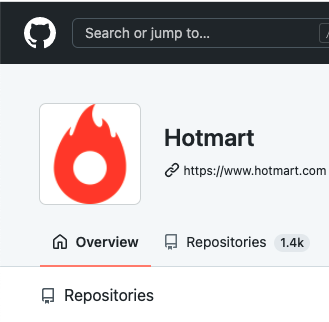
\includegraphics[scale=0.60,keepaspectratio=true]{images/01.png}
    \caption{Processo de maturidade}
    \label{pic_01}
\end{figure}

Na Figura \ref{pic_01}, podemos perceber como a oscilação das escolhas eram muito maiores antes de atingir o ponto de maturidade do que são a partir do momento em que já sabem qual caminho deseja trilhar.

Se fosse possível escolher as melhores partes das escolhas que nos tiraram do ponto de origem e nos levaram ao ponto de maturidade? Este seria um processo chamado de consolidação do conhecimento. Veja na Figura \ref{pic_02}.

\begin{figure}[H]
    \centering
    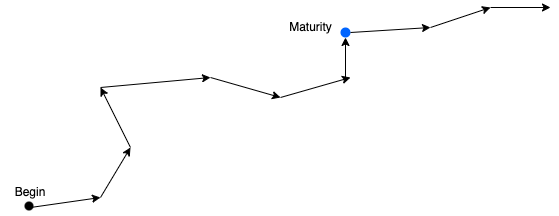
\includegraphics[scale=0.60,keepaspectratio=true]{images/02.png}
    \caption{Processo de consolidação do conhecimento}
    \label{pic_02}
\end{figure}

Agora, mesmo que soubéssemos as melhores escolhas, de nada adiantaria chegar até aqui sem a correta manutenção de cada delas, ou seja, sendo cada nova decisão deve-se levar em conta todas as demais.

\begin{figure}[H]
    \centering
    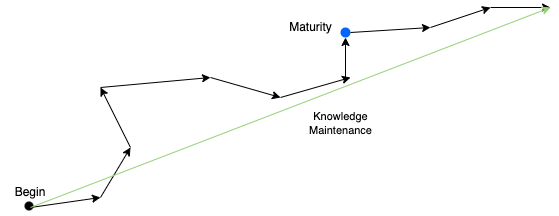
\includegraphics[scale=0.60,keepaspectratio=true]{images/03.png}
    \caption{Processo de manutenção do conhecimento}
    \label{pic_03}
\end{figure}

A cada passo de reconstrução, é muito importante documentar todas as etapas como por exemplo, regras de negócio, parâmetros e configurações e até mesmo um livro de receitas\footnote{playbook} que contem fragmentos de códigos que servem como referência futura. Quando temos uma referência em uma linha de produção, fica muito mais fácil garantir a qualidade de um produto.

Neste momento, estaríamos no que chamamos de \textbf{``Estado da Arte''} onde diversos setores da empresa poderiam trabalhar munidos de seus livros de receitas para execução de suas tarefas, entregando um trabalho de qualidade e deixando criatividade para ser utilizada no momento da criação de novos projetos ou seus incrementos.
\section{Start-Up ou não, Eis a Questão}

Muitas empresas intitulam-se como ``Start-Up'' sem saber de fato o que isso significa. Este termo pode estar relacionado à quantidade de pessoas que trabalham nela, ao baixo orçamento ou a ambiente de trabalho flexível, dentre outros.

Uma Start-Up também pode se caracterizar por seu \emph{modus operandi}, ou seja, um negócio possivelmente rentável mas que não atingiu maturidade suficiente para seguir com as próprias pernas e utiliza-se da estratégia \textbf{``erre rápido, conserte mais rápido ainda''}. 

Assim que uma Start-Up atinge seu nível de maturidade, ela começa a investir em pessoas e no ambiente de trabalho por saber que isso irá trazer bons resultados mas por que a Start-Up mas muitas vezes negligencia um dos ses maiores patrimônios, o software.

Talvez duas teorias possam ser plausíveis em casos como esses:
\begin{enumerate}
    \item O software é invisível: a empresa deve estar sempre vigilante para entender quando o software requer uma refatoração ou reconstrução.
    \item Time em que está ganhando não se mexe: essa é uma falácia pois sempre podemos melhorar um processo quando (i) revisamos o processo e o conseguimos melhorar ou quando (ii) não conseguimos melhorar o processo mas melhoramos nossa percepcão sobre ele. Ou seja, sempre há uma melhora.

\end{enumerate}
\section{O Monte Everest}

Em conversas com colegas de diferentes times, algumas certezas que sempre surgem são:
\begin{itemize}
    \item As regras de negócio nem sempre são claras;
    \item Não existe um controle de dependência para sabermos o que podemos alterar sem haver grandes efeitos colaterais;
    \item Vezes ou outras um time depende de atuar no código de outro time, o que demanda de mais atenção tanto de quem atua quanto de quem avalia os Pull Requests;
    \item Como não há um padrão bem definido, a qualidade do código fica  por conta daqueles que estão envolvidos no desenvolvimento;
\end{itemize}

Também em conversas com a turma, quando faço uma sugestão boba como ``e se determinada coisa fosse assim...'' os meus colegas me respondem mais ou menos assim ``seria um sonho, mas você sabe como as coisas são por aqui...'', ou seja, eles adorariam mas colocam tanta dificuldade que parece ser mais simples subir o Monte Everest do que executar qualquer mudança drástica por aqui.
% \section{O Poder do Conhecimento}

Confesso que toda essa situação me deixava inquieto e após muita reflexão, tentei buscar na internet alguma resposta. Dentre o jargão corporativo norte-americano temos o padrão $C(x)O \; | \; x \in [A...Z]$ como por exemplo \emph{CEO}\footnote{Chief of Executive Officer}, \emph{CTO}\footnote{Chief of Technology Officer}, \emph{CFO}\footnote{Chief of Financial Officer} e tantos outros. 

Mas o que me chamou mais a atenção foi o \textbf{K}, da \textbf{Chief Of Knowledge Officer}. Dentre suas atribuições, temos\footnote{https://searchcio.techtarget.com/definition/CKO}:

\begin{quotation}
    Diretor do conhecimento (CKO) é um título corporativo para a pessoa responsável por supervisionar a gestão do conhecimento dentro de uma organização. A posição do CKO está relacionada, mas é mais ampla do que a posição do CIO. A função do CKO é garantir que a empresa lucre com o uso eficaz dos recursos de conhecimento. Os investimentos em conhecimento podem incluir funcionários, processos e propriedade intelectual; um CKO pode ajudar uma organização a maximizar o retorno sobre o investimento (ROI) sobre esses investimentos.
    Além disso, um CKO pode ajudar uma organização a:
    \begin{itemize}
        \item Maximizar o retorno sobre o investimento (ROI) em conhecimento.
        \item Maximizar os benefícios de ativos intangíveis, como marca e relacionamento com o cliente.
        \item Repetir os sucessos, analise e aprendizagem com os fracassos.
        \item Promover as melhores práticas.
        \item Promover a inovação.
        \item Evitar a perda de conhecimento que pode resultar da perda de pessoal.
    \end{itemize}
\end{quotation}

Portanto, o que temos hoje como um mantra talvez pudesse formar o quarto pilar: O Pilar do Conhecimento. É muito mais fácil sustentar qualquer coisa com 4 pilares do que com apenas 3.

Uma característica bem interessante do Knowledge Officer é
\begin{quotation}
    \textbf{EXTRAIR O QUE AS PESSOAS TÊM DE MELHOR}
\end{quotation}
Ou seja, esse Novo Pilar além de estar sempre de braços abertos a toda e qualquer iniciativa, dando acolhimento e direcionamento adequado, pode contribuir para reescrever a missão da empresa, veja como:
\begin{quotation}
    \textbf{EXTRAIR O QUE AS PESSOAS TÊM DE MELHOR PARA PERMITIR QUE AS PESSOAS POSSAM VIVER DE SUAS PAIXÕES}
\end{quotation}

Isso seria excelência de ponta a ponta.

Para finalizar, para que tudo isso possa ser possível, seria necessária a criação de uma nova Torre, chamada de Torre do Conhecimento onde agregaria todos os Especialistas, Product Managers, Designers e Writers.
Essa Torre deveria receber as demandas da empresa, levantar requisitos, modelar entidades, elaboras layouts gráficos e textuais, e deve entregar um projeto no Jira já devidamente mensurado e organizado pronto para o time de desenvolvimento.

% 
\section{Metodologia para Reconstrução de Processos}

Uma vez ouvi a seguinte frase dita por Gustavo Caetano\footnote{CEO da SambaTech} que nunca mais saiu de minha mente:
\begin{quote}
    \textbf{SE} você me traz um problema \\
    \textbf{MAS} não me traz a solução \\
    \textbf{ENTÃO} você faz parte do problema
\end{quote}

Depois de refletir por muito tempo, entendi que nem sempre sabemos a solução de todos os problemas assim quando nos deparamos com eles e que  todos devem ser reportados imediatamente para mitigar quaisquer efeitos negativos. Por isso, adaptei essa frase para algo um pouco mais tangível:
\begin{quote}
    \textbf{SE} você me traz um problema \\
    \textbf{ENTÃO} vamos discutir uma solução \\
    \textbf{POIS} juntos trabalhamos melhor
\end{quote}

Baseado nessa frase, gostaria de apresentar uma metodologia ágil que estou desenvolvendo para reconstrução de processos maduros a qual batizei de \textbf{AIOROS}. Por mais caricata ou incomum que pareça, esta metodologia foi baseada na série japonesa de mangá e anime chamada \textbf{Os Cavaleiros do Zodíaco} veiculada no Brasil por volta dos anos 90.

Apesar de possuir diversas sagas, a primeira nos interessa por fazer uma analogia quase perfeita para o contexto que precisamos, onde os cavaleiros de bronze precisam salvar a princesa ferida, correndo contra to tempo, e para isso precisam passar pelas 12 casas do zodíaco enfrentando seus guardiões.

\begin{figure}[H]
    \centering
    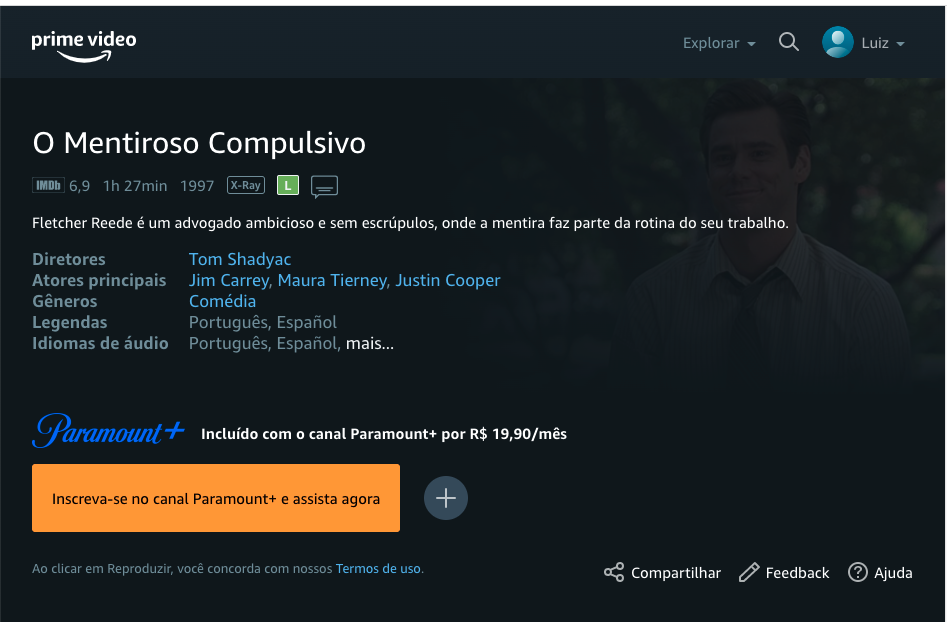
\includegraphics[scale=0.33,keepaspectratio=true]{images/06.png}
    \caption{Saori, reencarnação de Athena, ferida}
\end{figure}

Adaptando essa estória para nossa realidade, imagine que a princesa Saori seja a empresa ou o processo que está em execução de forma legada, ou seja, apenas com seu metabolismo basal não sendo capaz de entregar nada além do que suas funções básicas.

\begin{figure}[H]
    \centering
    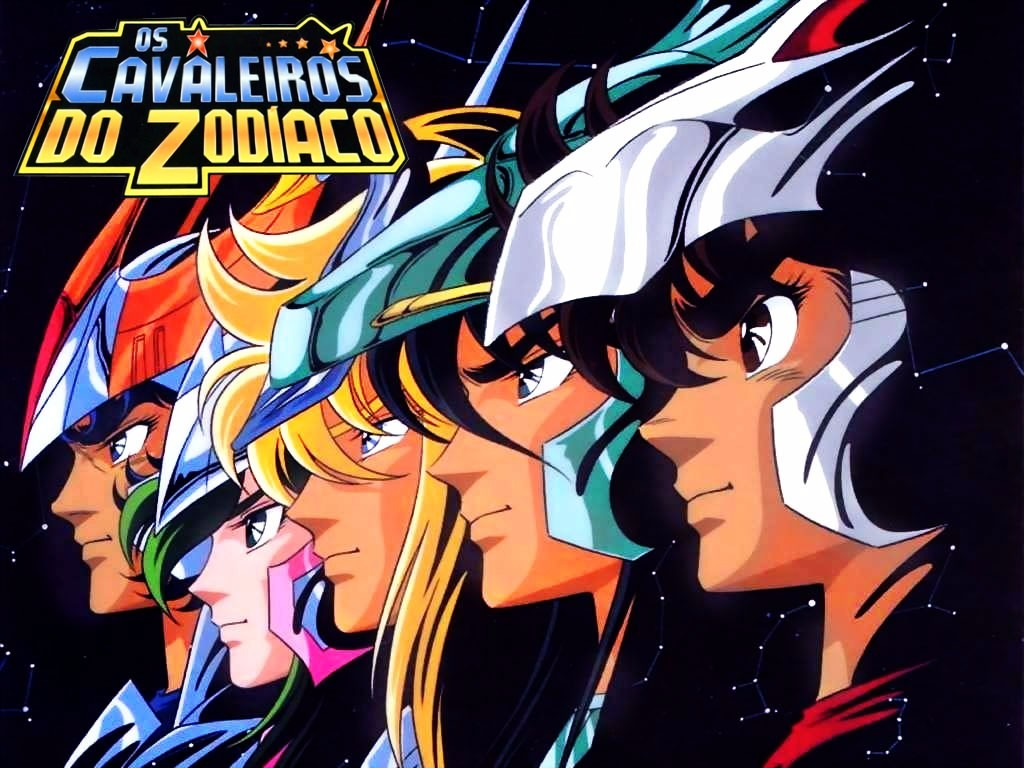
\includegraphics[scale=0.33,keepaspectratio=true]{images/05.jpg}
    \caption{Os Cavaleiros de Bronze}
\end{figure}

Já os cavaleiros de prata são os funcionários que reconhecem essa fraqueza nos processos legados e lutam arduamente em suas casas, enfrentando um guardião por vez.

\begin{figure}[H]
    \centering
    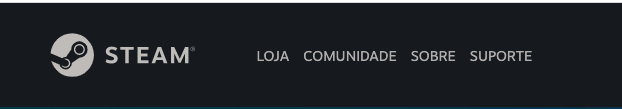
\includegraphics[scale=0.35,keepaspectratio=true]{images/07.png}
    \caption{Relógio das 12 casas do Zodíaco}
\end{figure}

O Relógio do Zodíaco a agilidade, ou seja, o time não tem muito tempo a perder pois processos e clientes aguardam ansiosamente por melhorias e o time deve trabalhar de forma integrada, coesa, a fim de garantir entregar dentro do prazo.

\begin{figure}[H]
    \centering
    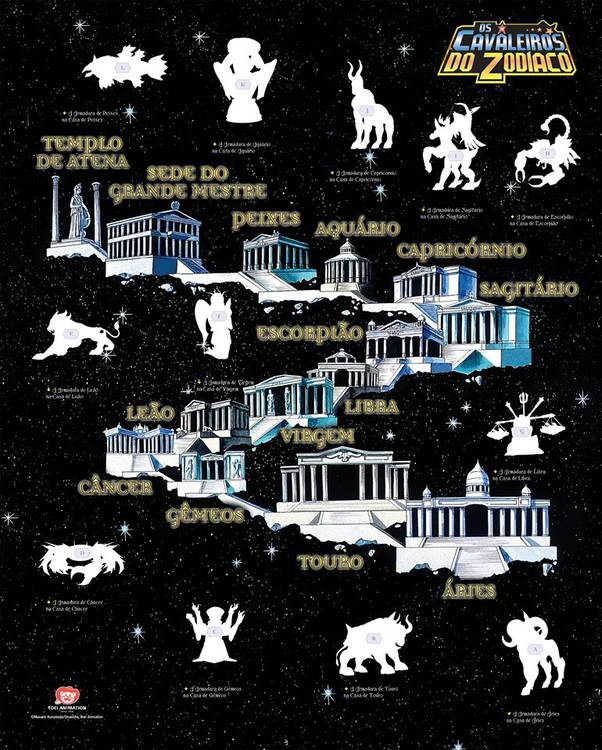
\includegraphics[scale=0.55,keepaspectratio=true]{images/08.jpg}
    \caption{As 12 casas do Zodíaco}
\end{figure}

As 12 Casas do Zodíaco representam em quantas partes o processo como um todo deverá ser quebrado. Deste ponto de vista, faz mais sentido dizer \textbf{As \emph{n} Casas do Zodíaco}. Mas aqui vale uma ressalva: 
\begin{itemize}
    \item Poucas casas deixam o sistema muito coeso, de difícil manutenção e com Cavaleiros de mais para combater
    \item Muitas casas deixar o sistema muito esparso, de difícil manutenção e com Cavaleiros de menos para combater
\end{itemize}

O segredo é ter uma equipe experiente para se definir qual é o número ideal de casas.

Portanto, vamos ver como isso funcionaria na prática
\begin{enumerate}
    \item Em uma reunião inicial a fim de explicar a todos os interessados o que será feito daqui pra frente;
    \item Em uma segunda reunião, de preferência com os membros mais experientes, deve-se de definir quais serão as casas a serem atacadas bem como nomear seus guardiões\footnote{deve-se haver pelo menos 2 guardiões para que haja uma cooperação mútua}
    \item Os guardiões, de posse de suas casas, devem definir os critérios de aceite e as regras de negócio que acharem pertinente à sua casa.
    \item Agora é a vez dos cavaleiros utilizarem do que há de melhor, elevando seus cosmos ao sétimo sentido, propondo soluções engenhosas que capazes de cobrir tudo que foi proposto pelos guardiões daquela casa. 
    \item Neste momento, Product Managers, Designers e Writers atuam ativamente na composição da solução do produto.
    \item Estes passos devem ser repetidos até que todo o projeto tenha finalizado. 
    \item Agora, Product Managers, Designers e Writers devem dar um formato no projeto, adicionando Epic, Estória, Tarefa, Sub-Tarefa para que os times executantes possam indicar o esforço para cada tarefa descrita. 
    \item Writers, não se esqueçam de que faz parte da entrega todas as chaves estarem traduzidas quando o projeto estiver fechado, ou seja, o time de desenvolvimento não poderá iniciar qualquer tarefa desde que essa condição não seja satisfeita. Essa entrega pode ser feita até via arquivo de texto anexado no card do jira, por exemplo.
    \item Voltando a falar sobre mensurar, como já teremos nosso livro de referência, teremos uma grande noção do quanto dura cada atividade, pelo menos uma boa aproximação. Dessa forma, fica bem mais simples e preciso saber quando uma tarefa deverá ser finalizada.
\end{enumerate}


\end{document}